\documentclass{article}
\usepackage[margin=1in]{geometry}
\usepackage{amsmath, amssymb}
\usepackage{hyperref}
\usepackage{graphicx}
\usepackage{enumitem}
\usepackage[square,numbers]{natbib}
\usepackage{setspace}

\title{LLM-Based Structurally Focused Topic Modeling (Draft)}
\author{Sam Mucyo}
\date{\today}

\begin{document}
\maketitle
\doublespacing

% ==========================
% Abstract
% ==========================
\begin{abstract}
    We investigate whether pre-extracting thematic elements via GPT-4 improves topic modeling by Latent Dirichlet Allocation (LDA) on Reddit mental-health posts. Using $\sim$10K documents from \texttt{r/depression} and \texttt{r/Anxiety}, we prompt GPT-4 to extract themes, emotional tone, cognitive patterns, and keywords, then compare LDA on structured text versus baseline processed text. We evaluate coherence ($c_v$), diversity, and perplexity; structured LDA shows a 25\% coherence gain and a 113\% perplexity reduction (4\% diversity loss). Qualitative pyLDAvis and word-cloud analyses confirm more interpretable topics. Code and data are at \url{https://github.com/Sam-Mucyo/neuro_and_ai}.
\end{abstract}

% ==========================
\section{Introduction}

Understanding the underlying themes within large collections of text is crucial for various academic, business, and research disciplines. Topic modeling is a well-established unsupervised technique used to automatically identify significant topics within a corpus. Traditional approaches, such as Latent Dirichlet Allocation (LDA), analyze patterns of word occurrences to identify these themes. While widely used, classic topic modeling approaches have certain drawbacks, including a potential lack of deep semantic understanding and the generation of topics that can be difficult for humans to interpret or distinguish without extensive post-processing. Assigning meaningful labels to topics based on word clusters is not always straightforward.

Recent advancements in Artificial Intelligence, particularly with the advent of Large Language Models (LLMs), have demonstrated unprecedented capabilities in understanding and generating human-like text. LLMs are transforming traditional Natural Language Processing (NLP) workflows. They can be used for various tasks, including text summarization, classification, and even potentially as alternatives to traditional topic modeling itself.

Inspired by these advancements and the potential to overcome the limitations of traditional methods, this project investigates a novel approach: leveraging the capabilities of LLMs to extract structured information from unstructured text \emph{before} applying traditional topic modeling techniques. This approach differs from using LLMs to generate topics directly or solely for post-processing tasks like topic labeling. Instead, the LLM acts as a sophisticated pre-processor, aiming to distill key structural or thematic elements from the text.

The central research question is:

\begin{center}
    \emph{Can LLM-driven structured extraction enhance Latent Dirichlet Allocation (LDA) topic modeling of natural language data, yielding more meaningful or insightful topics than conventional approaches?}
\end{center}

We hypothesize that incorporating structure extracted by an LLM will reveal latent themes tied to the data's organization. For example, in mental health discussions, we expect that an LLM can identify cognitive distortions, emotional tones, and specific concerns within posts. We hypothesize that running LDA on these structured outputs will produce clearer thematic groupings compared to running LDA directly on raw text. This approach was inspired by work analyzing educational video content that used LLMs to extract conceptual hierarchies before applying LDA to identify themes \citep{HramirEduConceptLibrarian}.

% ==========================
\section{Related Work}

Topic modeling has been a research topic of significant interest for many years. Traditional methods like Latent Dirichlet Allocation (LDA) \citep{Blei2003} analyze word co-occurrence patterns. While effective, they can produce topics that are collections of words not always intuitively meaningful or easily interpretable by humans. Preprocessing choices like stemming and lemmatization can also significantly affect performance.

The rise of LLMs has opened new avenues for text analysis. One line of work explores using LLMs \emph{directly} for topic extraction. The work by Mu \emph{et al.} investigates the potential of LLMs as a direct alternative to traditional topic modeling. Their framework prompts LLMs to generate topics from a given set of documents. They found that LLMs with appropriate prompts can generate relevant topic titles and adhere to guidelines for refining/merging topics. However, this direct generation approach can face challenges such as producing very general topics or highly overlapping topics, depending on prompting strategies and LLM capabilities.

Another related area uses LLMs to \emph{enhance} traditional topic modeling or text analysis workflows. The ``Unlocking insights from qualitative text with LLM-enhanced topic modeling'' source \citep{Bhaduri2024QualIT} describes QualIT, a tool that integrates pretrained LLMs with traditional clustering techniques. QualIT uses an LLM for initial key-phrase extraction from documents. These extracted key phrases are then clustered in a two-stage hierarchical process to identify overarching themes and more granular subtopics. This approach demonstrated improvements in topic coherence and diversity compared to standard LDA and BERTopic on benchmark datasets. Notably, QualIT leverages the LLM to extract structured information \emph{before} the clustering step. We also draw on an unpublished study on LLM-based topic modeling \citep{Mu2024LLM}, which investigates similar preprocessing pipelines.

Our project builds upon a similar principle of using LLMs for preprocessing/structuring before applying a traditional method. The work inspiring this project, the ``educational\_concept\_librarian'', used LLMs (specifically GPT) to extract conceptual hierarchies (graphs) from educational video transcripts. They then used these extracted graphs as the basis for feature extraction methods, including LDA applied to the concept graphs, to analyze content quality. This approach aligns closely with our methodology of using LLM-extracted structure as input for LDA.

While previous work has explored using LLMs as assistants for topic modeling (e.g., for evaluation or labeling) or using them directly for topic extraction, our approach focuses specifically on the strategy of using LLM-driven structured extraction as a deliberate step \emph{before} applying a traditional method like LDA, aiming to provide a more focused and potentially more interpretable input for the topic modeling algorithm. We then apply this specifically to mental health posts to see if similar trends are found.

% ==========================
\section{Methods}
We follow four compact steps:
\begin{enumerate}[leftmargin=*]
    \item \textbf{Data Preprocessing:} Clean and lemmatize raw posts using spaCy and NLTK.
    \item \textbf{Structured Extraction:} Prompt GPT-4 to produce JSON with themes, emotional tone, cognitive patterns, and keywords (schema in Appendix~A).
    \item \textbf{LDA Modeling:} Train two Gensim LDA models (10 topics, 20 passes, alpha='auto') on (a) structured text and (b) baseline processed text.
    \item \textbf{Evaluation:} Compute coherence ($c_v$), topic diversity, and perplexity; supplement results with pyLDAvis and word clouds.
\end{enumerate}

% ==========================
\section{Results}
\subsection{Quantitative Evaluation Metrics}

\begin{figure}[ht]
    \centering
    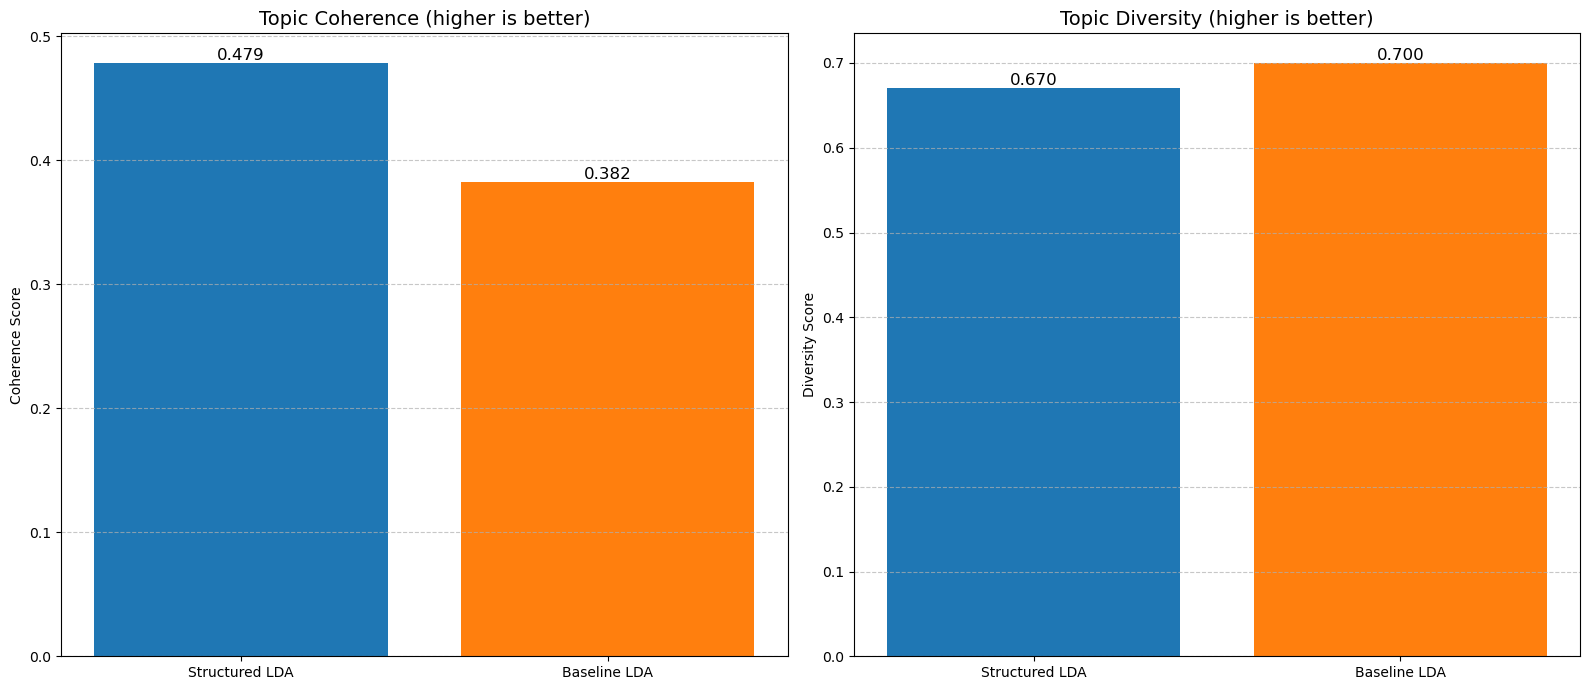
\includegraphics[width=0.7\textwidth]{plots/coherence_and_diversity_plots.png}
    \caption{Comparison of topic coherence ($c_v$) and diversity between Structured and Baseline LDA models.}
    \label{fig:coherence-diversity}
\end{figure}

\begin{figure}[ht]
    \centering
    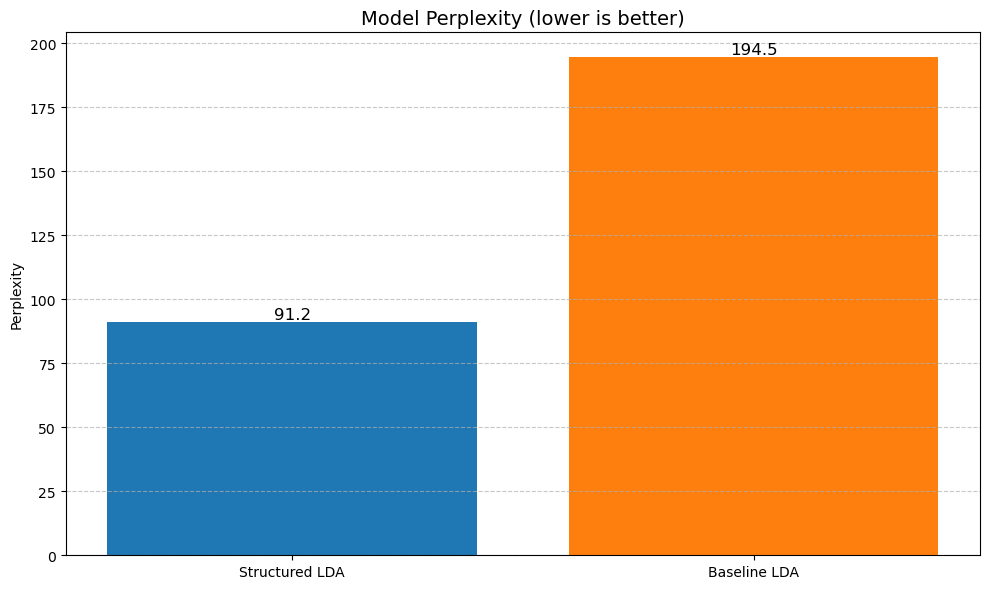
\includegraphics[width=0.7\textwidth]{plots/perplexity_plot.png}
    \caption{Comparison of model perplexity for Structured vs. Baseline LDA.}
    \label{fig:perplexity}
\end{figure}

The quantitative metrics demonstrate a notable difference between the two approaches. Figures~\ref{fig:coherence-diversity} and \ref{fig:perplexity} illustrate the results (see Appendix~\ref{app:metrics} for exact values).

\subsection{Qualitative Analysis}
The qualitative assessment through topic word clouds provided further insights into the nature of the topics generated by each approach.

% Word cloud figures
\begin{figure}[ht]
    \centering
    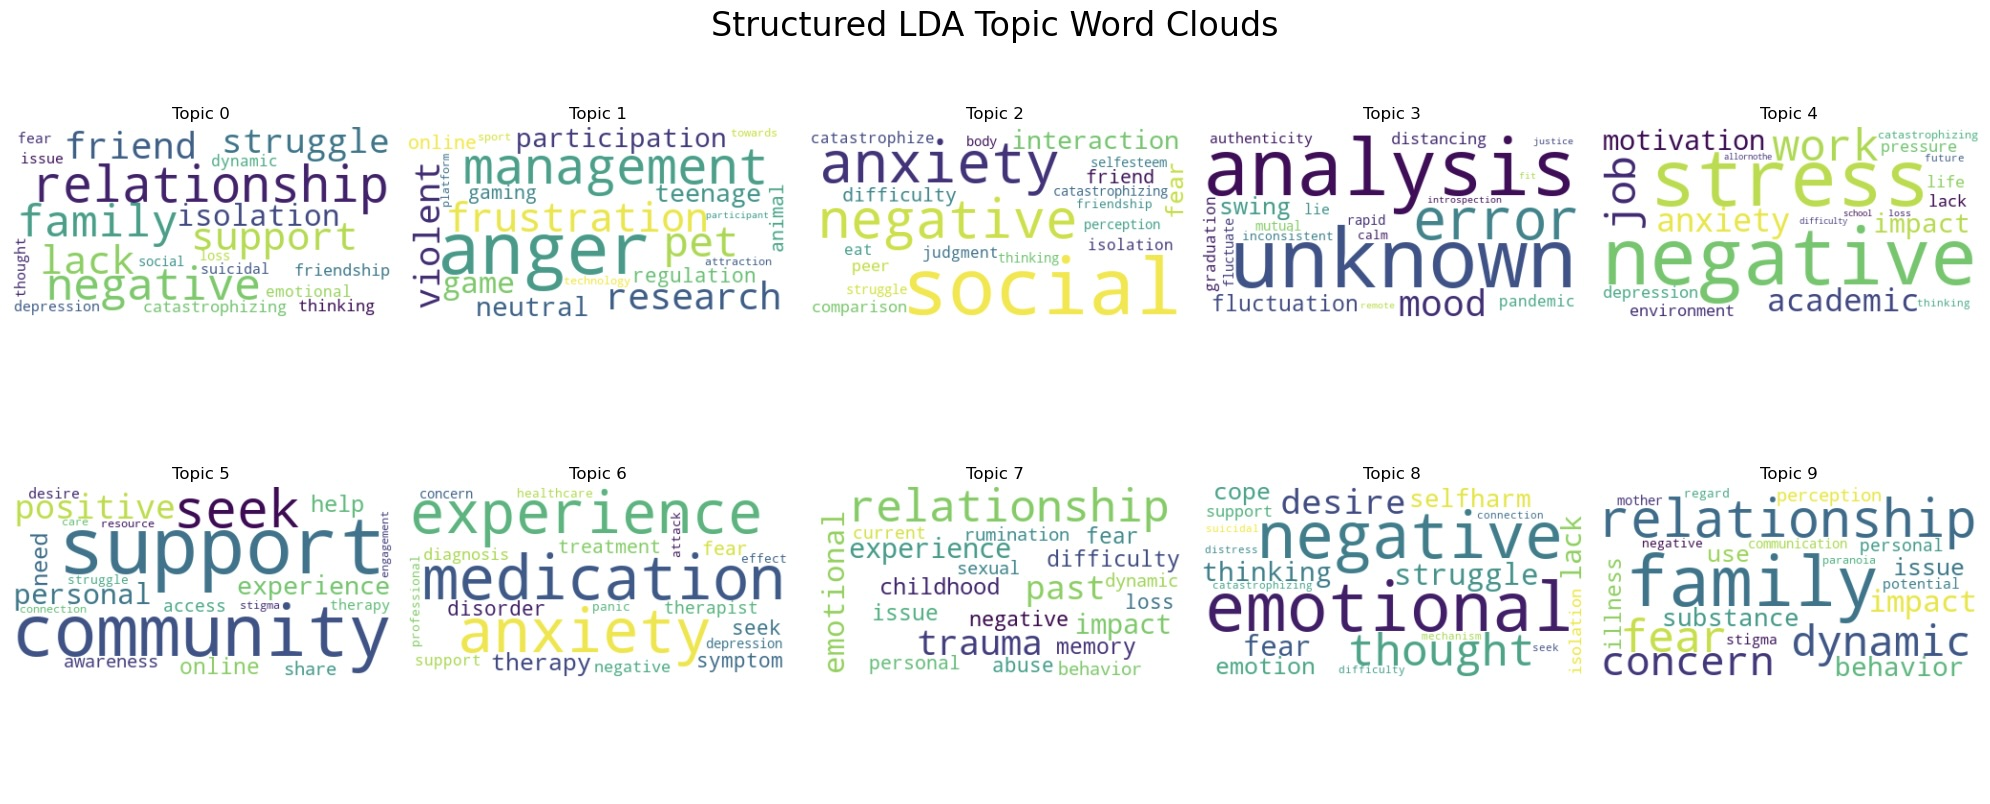
\includegraphics[width=0.8\textwidth]{plots/structuredLDATopicWordClouds.jpeg}
    \caption{Word clouds for topics generated by the Structured LDA model.}
    \label{fig:wordcloud-structured}
\end{figure}

\begin{figure}[ht]
    \centering
    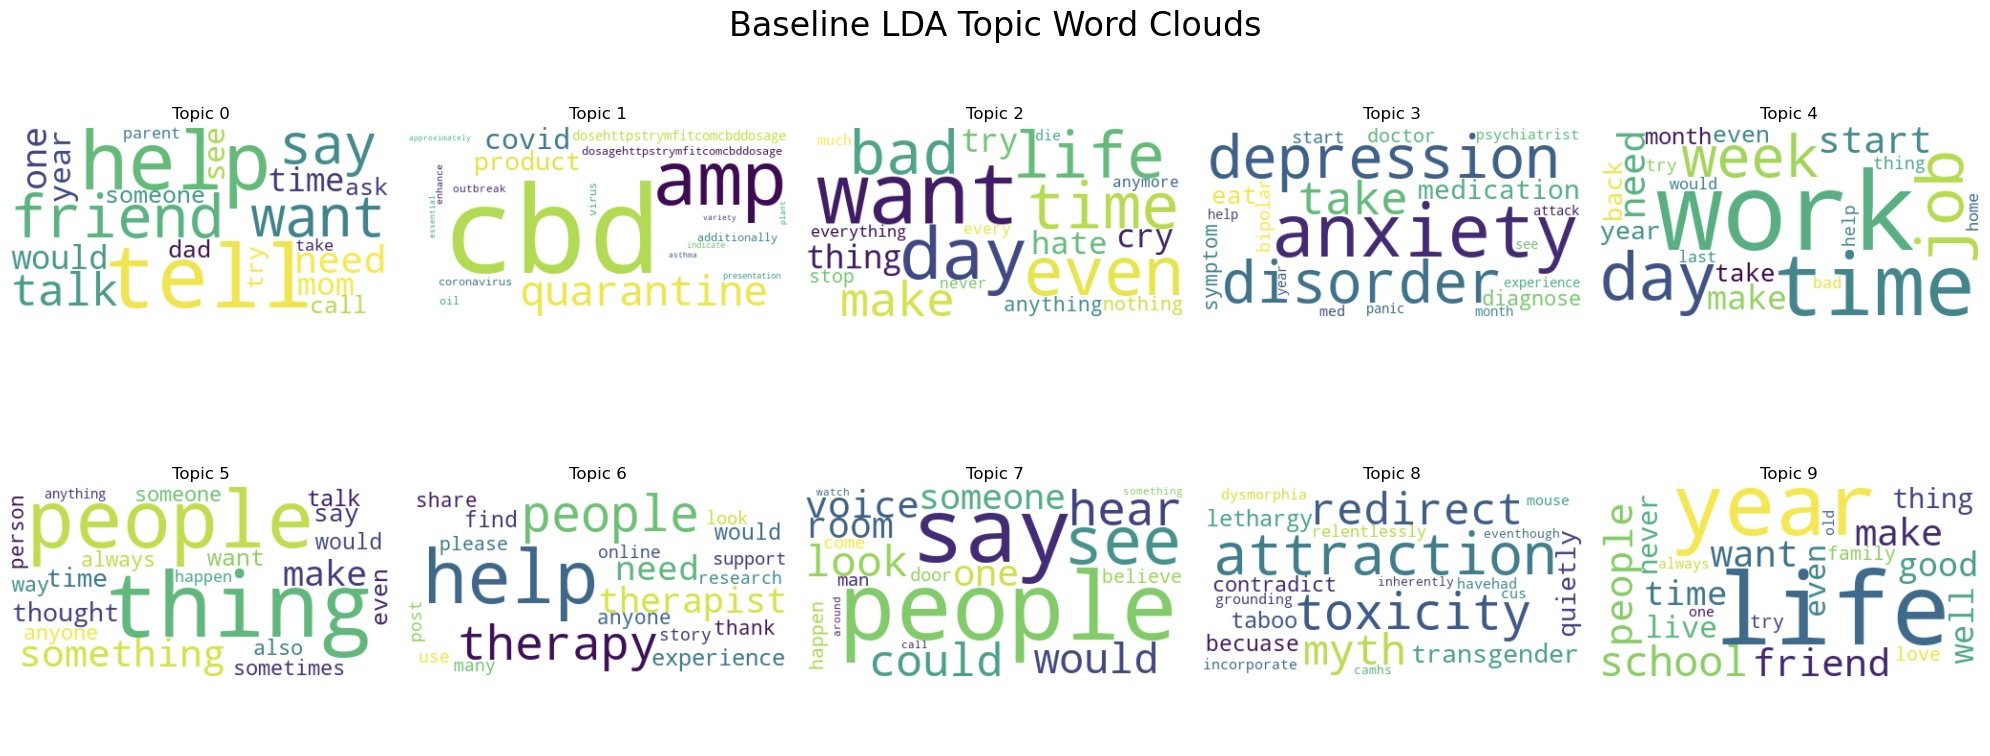
\includegraphics[width=0.8\textwidth]{plots/BaselineLDATopicWordClouds.jpeg}
    \caption{Word clouds for topics generated by the Baseline LDA model.}
    \label{fig:wordcloud-baseline}
\end{figure}

Reviewing the topic word clouds and the printed topics (list of top words):
\begin{itemize}[leftmargin=*]
    \item \textbf{Structured LDA} produced topics that appeared \emph{relatively distinct and interpretable}. The words within each topic seemed thematically related, making the underlying themes easier to understand. Examples of themes captured included topics focused on relationships/family/support, anger/frustration management, social anxiety, work/academic stress, and medication/therapy.
    \item \textbf{Baseline LDA} topics seemed \emph{less distinct and potentially harder to interpret}. They often featured very common words prominently (e.g., ``tell'', ``help'', ``want'', ``day'', ``time'', ``thing'', ``people''), which obscured specific themes. The overlap of common words suggested the baseline model struggled to separate themes as effectively as the structured approach. Some baseline topics contained seemingly unrelated words, making them less coherent subjectively.
\end{itemize}

The pyLDAvis plots show the inter-topic distance and the most salient terms. For the Structured LDA, the topic clusters appeared more distinct compared to the Baseline LDA, where some clusters seemed less separated. Interactive pyLDAvis visualizations for both Structured and Baseline LDA models are available online at \url{https://sammucyo.com/neuro140/}, where readers can explore inter-topic distance maps and term distributions.


% \textbf{TODO:} Include examples of representative documents for one or two topics from the Structured LDA, showing both the structured text and the original text. Discuss how the structured text captures key elements and how these relate to the identified topic.

Overall, the qualitative analysis visually and subjectively supports the quantitative findings that the Structured LDA approach generated topics that were \textbf{more coherent, interpretable, and distinct}.

% ==========================
\section{Discussion}

The results of this study provide compelling evidence supporting our hypothesis: \textbf{LLM-driven structured extraction can significantly enhance Latent Dirichlet Allocation (LDA) topic modeling, yielding more meaningful and insightful topics}. The quantitative metrics, particularly the substantial improvements in topic coherence (+25.19\%) and perplexity (+113.22\%) for the Structured LDA model, strongly indicate that feeding LDA with LLM-extracted structured information results in a statistically better topic distribution compared to using preprocessed raw text.

The qualitative findings reinforce this conclusion. The topics generated by the Structured LDA were consistently more interpretable and conceptually distinct, with words that clearly related to specific themes like relationships, anxiety, stress, or treatment. This contrasts with the Baseline LDA, whose topics were often dominated by general, high-frequency words that made specific thematic interpretation challenging.

Why does this approach work? By prompting the LLM to extract specific categories of information, such as themes, emotions, and cognitive patterns, we are essentially creating a more focused and relevant input for the LDA algorithm. The LLM acts as a powerful filter and distiller, reducing the noise present in raw text and surfacing the core elements relevant to mental health discussions. This pre-structuring step aligns with our hypothesis that incorporating structure would ``reveal latent themes tied to the data's organization''. The LDA algorithm, operating on this cleaner, structured representation, is better able to identify and separate underlying thematic groupings.

Our approach sits within a broader landscape of leveraging LLMs for text analysis. Unlike methods that use LLMs to \emph{directly} generate topics, our method integrates the LLM as a pre-processing step for a traditional algorithm. This hybrid approach allows us to benefit from the LLM's deep language understanding while still utilizing the well-understood probabilistic framework of LDA. It also offers a potential way to mitigate some challenges noted in direct LLM topic extraction, such as controlling topic granularity or handling overlapping topics, by shifting the clustering task to LDA. Our method also relates to initiatives like QualIT, which uses LLMs for key phrase extraction before clustering, but differs in the \emph{type} of structured information extracted (broader thematic/emotional categories vs. specific key phrases).

The success on this mental health dataset suggests that this ``Structurally Focused Topic Modeling'' approach could be particularly valuable in domains where identifying specific types of information or structural elements is key to understanding the data.

However, it is important to acknowledge limitations. The results were obtained on a specific dataset under controlled conditions, and performance may vary on different types of text or domains. The reliability and consistency of the LLM's structured output is paramount and requires careful prompt engineering and potential validation. While the diversity metric was slightly lower for the Structured LDA, this decrease (-4.29\%) may be a trade-off for significantly increased coherence and interpretability, which are often considered more crucial for understanding the topics. Further research could explore how to optimize for both coherence and diversity simultaneously in this framework. The choice of the number of topics ($K$) for LDA also influences the results, and while coherence analysis can guide this, it remains a parameter to be tuned.

% ==========================
\section{Conclusion and Future Work}
This study successfully demonstrated that integrating LLM-driven structured extraction into a traditional LDA topic modeling pipeline significantly enhances the quality and interpretability of the resulting topics on a mental health discussion dataset. By transforming unstructured text into a semi-structured format based on key thematic elements, emotions, and cognitive patterns, the LDA model was able to identify more coherent and distinct themes than when applied to raw text. The substantial improvements in topic coherence and perplexity, supported by the qualitative analysis of topic interpretability, validate our hypothesis.

This work highlights the potential of using LLMs not just as standalone models but as powerful components within multi-step text analysis workflows. This hybrid approach offers a promising direction for gaining deeper insights from complex natural language data in various domains.

For future work, we plan to expand our experiments to include datasets from different domains to assess the generalizability of this methodology. Further refinement of the LLM prompt and exploring different LLM models or variations in the extracted structured features could potentially lead to even better results. Comparing this approach to other state-of-the-art topic modeling methods (e.g., BERTopic) or methods using LLMs differently (e.g., direct topic generation) would provide a more comprehensive understanding of its strengths and weaknesses. Addressing the challenge of processing very long documents that exceed LLM context windows is also an important area for future research. Finally, conducting a formal human evaluation of topic quality would provide a more rigorous subjective assessment.

% ==========================
\bibliographystyle{plainnat}
\bibliography{references}

% ==========================
\section*{Code and Data Availability}
The complete code, processed data (\texttt{results/processed\_data.csv}), and analysis notebooks are available at \url{https://github.com/Sam-Mucyo/neuro_and_ai}.

\appendix
\section{Detailed JSON Prompt Schema}
\label{app:prompt-schema}
\begin{verbatim}
{
  "type": "object",
  "properties": {
    "themes": {"type": "array", "items": {"type": "string"}},
    "emotional_tone": {"type": "string", "enum": ["positive", "negative", "neutral", "mixed", "unknown"]},
    "concerns": {"type": "array", "items": {"type": "string"}},
    "cognitive_patterns": {"type": "array", "items": {"type": "string"}},
    "social_context": {"type": "array", "items": {"type": "string"}}
  },
  "required": ["themes","emotional_tone","concerns","cognitive_patterns","social_context"],
  "additionalProperties": false
}
\end{verbatim}

\section{Quantitative Evaluation Table}
\label{app:metrics}
\begin{table}[ht]
    \centering
    \begin{tabular}{lccc}
        \hline
        Approach       & Coherence ($c_v$) & Diversity & Perplexity \\
        \hline
        Structured LDA & 0.478549          & 0.67      & 91.214453  \\
        Baseline LDA   & 0.382260          & 0.70      & 194.484527 \\
        \hline
    \end{tabular}
    \caption{Exact quantitative evaluation metrics for Structured vs. Baseline LDA models.}
    \label{tab:metrics-app}
\end{table}

\end{document}
